\documentclass[a4paper]{book}
\usepackage{a4wide}
\usepackage{makeidx}
\usepackage{fancyhdr}
\usepackage{graphicx}
\usepackage{multicol}
\usepackage{float}
\usepackage{textcomp}
\usepackage{alltt}
\usepackage{times}
\usepackage{ifpdf}
\ifpdf
\usepackage[pdftex,
            pagebackref=true,
            colorlinks=true,
            linkcolor=blue,
            unicode
           ]{hyperref}
\else
\usepackage[ps2pdf,
            pagebackref=true,
            colorlinks=true,
            linkcolor=blue,
            unicode
           ]{hyperref}
\usepackage{pspicture}
\fi
\usepackage[utf8]{inputenc}
\usepackage{doxygen}
\makeindex
\setcounter{tocdepth}{3}
\renewcommand{\footrulewidth}{0.4pt}
\begin{document}
\begin{titlepage}
\vspace*{7cm}
\begin{center}
{\Large libusock \\[1ex]\large 0.1b }\\
\vspace*{1cm}
{\large Generated by Doxygen 1.5.7}\\
\vspace*{0.5cm}
{\small Thu May 14 11:19:36 2009}\\
\end{center}
\end{titlepage}
\clearemptydoublepage
\pagenumbering{roman}
\tableofcontents
\clearemptydoublepage
\pagenumbering{arabic}
\chapter{Class Index}
\section{Class Hierarchy}
This inheritance list is sorted roughly, but not completely, alphabetically:\begin{CompactList}
\item \contentsline{section}{icmp\_\-hdr}{\pageref{structicmp__hdr}}{}
\item \contentsline{section}{pseudohdr}{\pageref{structpseudohdr}}{}
\item \contentsline{section}{Socket}{\pageref{classSocket}}{}
\begin{CompactList}
\item \contentsline{section}{RawSocket}{\pageref{classRawSocket}}{}
\item \contentsline{section}{ServerSocket}{\pageref{classServerSocket}}{}
\item \contentsline{section}{UDPSocket}{\pageref{classUDPSocket}}{}
\end{CompactList}
\item \contentsline{section}{SocketException}{\pageref{classSocketException}}{}
\end{CompactList}

\chapter{Class Index}
\section{Class List}
Here are the classes, structs, unions and interfaces with brief descriptions:\begin{CompactList}
\item\contentsline{section}{\hyperlink{structicmp__hdr}{icmp\_\-hdr} }{\pageref{structicmp__hdr}}{}
\item\contentsline{section}{\hyperlink{structpseudohdr}{pseudohdr} }{\pageref{structpseudohdr}}{}
\item\contentsline{section}{\hyperlink{classRawSocket}{RawSocket} (Class for managing raw sockets )}{\pageref{classRawSocket}}{}
\item\contentsline{section}{\hyperlink{classServerSocket}{ServerSocket} (Class for managing server sockets )}{\pageref{classServerSocket}}{}
\item\contentsline{section}{\hyperlink{classSocket}{Socket} (Base socket class for building, by default, TCP sockets )}{\pageref{classSocket}}{}
\item\contentsline{section}{\hyperlink{classSocketException}{SocketException} }{\pageref{classSocketException}}{}
\item\contentsline{section}{\hyperlink{classUDPSocket}{UDPSocket} (Class for managing UDP sockets )}{\pageref{classUDPSocket}}{}
\end{CompactList}

\chapter{File Index}
\section{File List}
Here is a list of all files with brief descriptions:\begin{CompactList}
\item\contentsline{section}{\hyperlink{usock_8h}{usock.h} }{\pageref{usock_8h}}{}
\item\contentsline{section}{\hyperlink{usock__exception_8h}{usock\_\-exception.h} }{\pageref{usock__exception_8h}}{}
\end{CompactList}

\chapter{Class Documentation}
\hypertarget{structicmp__hdr}{
\section{icmp\_\-hdr Struct Reference}
\label{structicmp__hdr}\index{icmp\_\-hdr@{icmp\_\-hdr}}
}
{\tt \#include $<$usock.h$>$}

\subsection*{Public Attributes}
\begin{CompactItemize}
\item 
u\_\-int8\_\-t \hyperlink{structicmp__hdr_054d3b022febf3b05f1ddb9dd906dbfa}{type}
\item 
u\_\-int8\_\-t \hyperlink{structicmp__hdr_20c797dc348a3a620929169f5637515f}{code}
\item 
u\_\-int16\_\-t \hyperlink{structicmp__hdr_adfc592902141c82e5feda1c26c8f1cc}{checksum}
\item 
u\_\-int16\_\-t \hyperlink{structicmp__hdr_8ceada44796f077ba4398312b65aa6e5}{id}
\item 
u\_\-int16\_\-t \hyperlink{structicmp__hdr_747445ef1c8275eccce121fd1a5f5b90}{sequence}
\end{CompactItemize}


\subsection{Member Data Documentation}
\hypertarget{structicmp__hdr_adfc592902141c82e5feda1c26c8f1cc}{
\index{icmp\_\-hdr@{icmp\_\-hdr}!checksum@{checksum}}
\index{checksum@{checksum}!icmp_hdr@{icmp\_\-hdr}}
\subsubsection[{checksum}]{\setlength{\rightskip}{0pt plus 5cm}u\_\-int16\_\-t {\bf icmp\_\-hdr::checksum}}}
\label{structicmp__hdr_adfc592902141c82e5feda1c26c8f1cc}


\hypertarget{structicmp__hdr_20c797dc348a3a620929169f5637515f}{
\index{icmp\_\-hdr@{icmp\_\-hdr}!code@{code}}
\index{code@{code}!icmp_hdr@{icmp\_\-hdr}}
\subsubsection[{code}]{\setlength{\rightskip}{0pt plus 5cm}u\_\-int8\_\-t {\bf icmp\_\-hdr::code}}}
\label{structicmp__hdr_20c797dc348a3a620929169f5637515f}


\hypertarget{structicmp__hdr_8ceada44796f077ba4398312b65aa6e5}{
\index{icmp\_\-hdr@{icmp\_\-hdr}!id@{id}}
\index{id@{id}!icmp_hdr@{icmp\_\-hdr}}
\subsubsection[{id}]{\setlength{\rightskip}{0pt plus 5cm}u\_\-int16\_\-t {\bf icmp\_\-hdr::id}}}
\label{structicmp__hdr_8ceada44796f077ba4398312b65aa6e5}


\hypertarget{structicmp__hdr_747445ef1c8275eccce121fd1a5f5b90}{
\index{icmp\_\-hdr@{icmp\_\-hdr}!sequence@{sequence}}
\index{sequence@{sequence}!icmp_hdr@{icmp\_\-hdr}}
\subsubsection[{sequence}]{\setlength{\rightskip}{0pt plus 5cm}u\_\-int16\_\-t {\bf icmp\_\-hdr::sequence}}}
\label{structicmp__hdr_747445ef1c8275eccce121fd1a5f5b90}


\hypertarget{structicmp__hdr_054d3b022febf3b05f1ddb9dd906dbfa}{
\index{icmp\_\-hdr@{icmp\_\-hdr}!type@{type}}
\index{type@{type}!icmp_hdr@{icmp\_\-hdr}}
\subsubsection[{type}]{\setlength{\rightskip}{0pt plus 5cm}u\_\-int8\_\-t {\bf icmp\_\-hdr::type}}}
\label{structicmp__hdr_054d3b022febf3b05f1ddb9dd906dbfa}




The documentation for this struct was generated from the following file:\begin{CompactItemize}
\item 
\hyperlink{usock_8h}{usock.h}\end{CompactItemize}

\hypertarget{structpseudohdr}{
\section{pseudohdr Struct Reference}
\label{structpseudohdr}\index{pseudohdr@{pseudohdr}}
}
{\tt \#include $<$usock.h$>$}

\subsection*{Public Attributes}
\begin{CompactItemize}
\item 
u\_\-int32\_\-t \hyperlink{structpseudohdr_c5ae2d59641e771ad3b48a6c29158a87}{src}
\item 
u\_\-int32\_\-t \hyperlink{structpseudohdr_ee1762538b3aaf3d81c7475461795570}{dst}
\item 
u\_\-int8\_\-t \hyperlink{structpseudohdr_c3318d4b453ac87a82cdaa8e384b7bfe}{padd}
\item 
u\_\-int8\_\-t \hyperlink{structpseudohdr_52550c6d13a3557d8d3a947d83f362f6}{proto}
\item 
u\_\-int16\_\-t \hyperlink{structpseudohdr_cb0c71af98d9bd008085860cdb4b43a4}{len}
\end{CompactItemize}


\subsection{Member Data Documentation}
\hypertarget{structpseudohdr_ee1762538b3aaf3d81c7475461795570}{
\index{pseudohdr@{pseudohdr}!dst@{dst}}
\index{dst@{dst}!pseudohdr@{pseudohdr}}
\subsubsection[{dst}]{\setlength{\rightskip}{0pt plus 5cm}u\_\-int32\_\-t {\bf pseudohdr::dst}}}
\label{structpseudohdr_ee1762538b3aaf3d81c7475461795570}


\hypertarget{structpseudohdr_cb0c71af98d9bd008085860cdb4b43a4}{
\index{pseudohdr@{pseudohdr}!len@{len}}
\index{len@{len}!pseudohdr@{pseudohdr}}
\subsubsection[{len}]{\setlength{\rightskip}{0pt plus 5cm}u\_\-int16\_\-t {\bf pseudohdr::len}}}
\label{structpseudohdr_cb0c71af98d9bd008085860cdb4b43a4}


\hypertarget{structpseudohdr_c3318d4b453ac87a82cdaa8e384b7bfe}{
\index{pseudohdr@{pseudohdr}!padd@{padd}}
\index{padd@{padd}!pseudohdr@{pseudohdr}}
\subsubsection[{padd}]{\setlength{\rightskip}{0pt plus 5cm}u\_\-int8\_\-t {\bf pseudohdr::padd}}}
\label{structpseudohdr_c3318d4b453ac87a82cdaa8e384b7bfe}


\hypertarget{structpseudohdr_52550c6d13a3557d8d3a947d83f362f6}{
\index{pseudohdr@{pseudohdr}!proto@{proto}}
\index{proto@{proto}!pseudohdr@{pseudohdr}}
\subsubsection[{proto}]{\setlength{\rightskip}{0pt plus 5cm}u\_\-int8\_\-t {\bf pseudohdr::proto}}}
\label{structpseudohdr_52550c6d13a3557d8d3a947d83f362f6}


\hypertarget{structpseudohdr_c5ae2d59641e771ad3b48a6c29158a87}{
\index{pseudohdr@{pseudohdr}!src@{src}}
\index{src@{src}!pseudohdr@{pseudohdr}}
\subsubsection[{src}]{\setlength{\rightskip}{0pt plus 5cm}u\_\-int32\_\-t {\bf pseudohdr::src}}}
\label{structpseudohdr_c5ae2d59641e771ad3b48a6c29158a87}




The documentation for this struct was generated from the following file:\begin{CompactItemize}
\item 
\hyperlink{usock_8h}{usock.h}\end{CompactItemize}

\hypertarget{classRawSocket}{
\section{RawSocket Class Reference}
\label{classRawSocket}\index{RawSocket@{RawSocket}}
}
Class for managing raw sockets.  


{\tt \#include $<$usock.h$>$}

Inheritance diagram for RawSocket::\begin{figure}[H]
\begin{center}
\leavevmode
\includegraphics[height=2cm]{classRawSocket}
\end{center}
\end{figure}
\subsection*{Public Member Functions}
\begin{CompactItemize}
\item 
\hyperlink{classRawSocket_10fc562aa855e7f4b184af1d4f842ae0}{RawSocket} (std::string i=\char`\"{}lo\char`\"{})
\begin{CompactList}\small\item\em \hyperlink{classRawSocket}{RawSocket} constructor. \item\end{CompactList}\item 
std::string \hyperlink{classRawSocket_dda64a716b48c1527283c026bda208d6}{getIPv4addr} ()  throw ()
\begin{CompactList}\small\item\em Get the IPv4 address associated to the network interface. \item\end{CompactList}\item 
std::string \hyperlink{classRawSocket_b35260c4a551194b50925537785bcf47}{getHWaddr} ()  throw ()
\begin{CompactList}\small\item\em Get the HW address associated to the network interface. \item\end{CompactList}\item 
u\_\-int16\_\-t \hyperlink{classRawSocket_973b337d963bdcff3ce68d0ef7ffb7e1}{csum} (u\_\-int16\_\-t $\ast$buf, int nwords)
\begin{CompactList}\small\item\em Compute the checksum of a buffer. \item\end{CompactList}\item 
void \hyperlink{classRawSocket_9536928bd82c99ef2b615b0ffcb87f21}{buildIPv4} (std::string dst, std::string src=\char`\"{}\char`\"{}, u\_\-int8\_\-t proto=IPPROTO\_\-TCP, u\_\-int16\_\-t len=0, u\_\-int8\_\-t ttl=32, u\_\-int8\_\-t tos=0, u\_\-int16\_\-t id=0, u\_\-int16\_\-t frag=0, u\_\-int16\_\-t sum=0)
\begin{CompactList}\small\item\em Build an IPv4 header for the raw socket. \item\end{CompactList}\item 
void \hyperlink{classRawSocket_ba3cca3e8ff995d5edbf064b3af8ca05}{buildTCP} (u\_\-int16\_\-t sport, u\_\-int16\_\-t dport, u\_\-int8\_\-t flags, u\_\-int32\_\-t seq=0, u\_\-int32\_\-t ack=0, u\_\-int16\_\-t window=0x1000, u\_\-int16\_\-t urgent=0, u\_\-int16\_\-t sum=0)
\begin{CompactList}\small\item\em Build a TCP header for the raw socket. \item\end{CompactList}\item 
void \hyperlink{classRawSocket_90915831a7ac1046e07635da346a54fe}{buildUDP} (u\_\-int16\_\-t sport, u\_\-int16\_\-t dport, u\_\-int16\_\-t len=0, u\_\-int16\_\-t sum=0)
\begin{CompactList}\small\item\em Build an UDP header for the raw socket. \item\end{CompactList}\item 
void \hyperlink{classRawSocket_07d676b2f5becf9fad465b7f63f9d3a3}{buildICMPv4} (u\_\-int8\_\-t \hyperlink{classSocket_c7f6980f36023df2004271c336217cb8}{type}, u\_\-int16\_\-t id=0x100, u\_\-int16\_\-t seq=0x100, u\_\-int8\_\-t code=0, u\_\-int16\_\-t sum=0)
\begin{CompactList}\small\item\em Build an ICMPv4 header for the raw socket. \item\end{CompactList}\item 
void \hyperlink{classRawSocket_4969ba6947943aed82dc3cebb5c0f708}{setPayload} (void $\ast$payload, int length)
\begin{CompactList}\small\item\em Set a binary payload for the raw socket. \item\end{CompactList}\item 
void \hyperlink{classRawSocket_2e97eed0b10d4f48012eedde25099fd1}{setPayload} (std::string payload)
\begin{CompactList}\small\item\em Set a payload for the raw socket as a string. \item\end{CompactList}\item 
void \hyperlink{classRawSocket_149999a5d231c93e206be89eec9732b8}{write} ()  throw ()
\begin{CompactList}\small\item\em Write the raw packet onto the network interface. \item\end{CompactList}\item 
void $\ast$ \hyperlink{classRawSocket_f41dd9eca89c3e4bb5c5bbf5af10dbd7}{read} (u\_\-int32\_\-t len, const std::string \&host=\char`\"{}\char`\"{})  throw ()
\begin{CompactList}\small\item\em Read binary data from the raw socket. \item\end{CompactList}\end{CompactItemize}


\subsection{Detailed Description}
Class for managing raw sockets. 

\begin{Desc}
\item[Author:]BlackLight \end{Desc}


\subsection{Constructor \& Destructor Documentation}
\hypertarget{classRawSocket_10fc562aa855e7f4b184af1d4f842ae0}{
\index{RawSocket@{RawSocket}!RawSocket@{RawSocket}}
\index{RawSocket@{RawSocket}!RawSocket@{RawSocket}}
\subsubsection[{RawSocket}]{\setlength{\rightskip}{0pt plus 5cm}RawSocket::RawSocket (std::string {\em i} = {\tt \char`\"{}lo\char`\"{}})}}
\label{classRawSocket_10fc562aa855e7f4b184af1d4f842ae0}


\hyperlink{classRawSocket}{RawSocket} constructor. 

\begin{Desc}
\item[Parameters:]
\begin{description}
\item[{\em i}]Interface on which we're going to bind our raw socket \end{description}
\end{Desc}


\subsection{Member Function Documentation}
\hypertarget{classRawSocket_07d676b2f5becf9fad465b7f63f9d3a3}{
\index{RawSocket@{RawSocket}!buildICMPv4@{buildICMPv4}}
\index{buildICMPv4@{buildICMPv4}!RawSocket@{RawSocket}}
\subsubsection[{buildICMPv4}]{\setlength{\rightskip}{0pt plus 5cm}void RawSocket::buildICMPv4 (u\_\-int8\_\-t {\em type}, \/  u\_\-int16\_\-t {\em id} = {\tt 0x100}, \/  u\_\-int16\_\-t {\em seq} = {\tt 0x100}, \/  u\_\-int8\_\-t {\em code} = {\tt 0}, \/  u\_\-int16\_\-t {\em sum} = {\tt 0})}}
\label{classRawSocket_07d676b2f5becf9fad465b7f63f9d3a3}


Build an ICMPv4 header for the raw socket. 

\begin{Desc}
\item[Parameters:]
\begin{description}
\item[{\em type}]ICMP type \item[{\em id}]Packet ID (default: 0x100) \item[{\em seq}]Sequence number (default: 0x100) \item[{\em code}]ICMP code (default: 0) \item[{\em sum}]ICMP checksum (default: auto-computed) \end{description}
\end{Desc}
\hypertarget{classRawSocket_9536928bd82c99ef2b615b0ffcb87f21}{
\index{RawSocket@{RawSocket}!buildIPv4@{buildIPv4}}
\index{buildIPv4@{buildIPv4}!RawSocket@{RawSocket}}
\subsubsection[{buildIPv4}]{\setlength{\rightskip}{0pt plus 5cm}void RawSocket::buildIPv4 (std::string {\em dst}, \/  std::string {\em src} = {\tt \char`\"{}\char`\"{}}, \/  u\_\-int8\_\-t {\em proto} = {\tt IPPROTO\_\-TCP}, \/  u\_\-int16\_\-t {\em len} = {\tt 0}, \/  u\_\-int8\_\-t {\em ttl} = {\tt 32}, \/  u\_\-int8\_\-t {\em tos} = {\tt 0}, \/  u\_\-int16\_\-t {\em id} = {\tt 0}, \/  u\_\-int16\_\-t {\em frag} = {\tt 0}, \/  u\_\-int16\_\-t {\em sum} = {\tt 0})}}
\label{classRawSocket_9536928bd82c99ef2b615b0ffcb87f21}


Build an IPv4 header for the raw socket. 

\begin{Desc}
\item[Parameters:]
\begin{description}
\item[{\em dst}]Destination hostname/address \item[{\em src}]Source hostname/address (default: IPv4 address associated to the network interface) \item[{\em proto}]Transport protocol (default: TCP) \item[{\em len}]Total length of the IPv4 datagram (default: header length + payload length) \item[{\em ttl}]Time To Live (default: 32) \item[{\em tos}]Type Of Service (default: 0) \item[{\em id}]Datagram ID (default: 0) \item[{\em frag}]Fragmentation flag (default: 0) \item[{\em sum}]IPv4 checksum (default: auto-computed) \end{description}
\end{Desc}
\hypertarget{classRawSocket_ba3cca3e8ff995d5edbf064b3af8ca05}{
\index{RawSocket@{RawSocket}!buildTCP@{buildTCP}}
\index{buildTCP@{buildTCP}!RawSocket@{RawSocket}}
\subsubsection[{buildTCP}]{\setlength{\rightskip}{0pt plus 5cm}void RawSocket::buildTCP (u\_\-int16\_\-t {\em sport}, \/  u\_\-int16\_\-t {\em dport}, \/  u\_\-int8\_\-t {\em flags}, \/  u\_\-int32\_\-t {\em seq} = {\tt 0}, \/  u\_\-int32\_\-t {\em ack} = {\tt 0}, \/  u\_\-int16\_\-t {\em window} = {\tt 0x1000}, \/  u\_\-int16\_\-t {\em urgent} = {\tt 0}, \/  u\_\-int16\_\-t {\em sum} = {\tt 0})}}
\label{classRawSocket_ba3cca3e8ff995d5edbf064b3af8ca05}


Build a TCP header for the raw socket. 

\begin{Desc}
\item[Parameters:]
\begin{description}
\item[{\em sport}]Source port \item[{\em dport}]Destination port \item[{\em flags}]TCP flags \item[{\em seq}]Sequence number (default: randomly generated) \item[{\em ack}]ACK number (default: 0) \item[{\em window}]Window size (default: 16) \item[{\em urgent}]Urgent pointer (default: 0) \item[{\em sum}]TCP checksum (default: auto-computed) \end{description}
\end{Desc}
\hypertarget{classRawSocket_90915831a7ac1046e07635da346a54fe}{
\index{RawSocket@{RawSocket}!buildUDP@{buildUDP}}
\index{buildUDP@{buildUDP}!RawSocket@{RawSocket}}
\subsubsection[{buildUDP}]{\setlength{\rightskip}{0pt plus 5cm}void RawSocket::buildUDP (u\_\-int16\_\-t {\em sport}, \/  u\_\-int16\_\-t {\em dport}, \/  u\_\-int16\_\-t {\em len} = {\tt 0}, \/  u\_\-int16\_\-t {\em sum} = {\tt 0})}}
\label{classRawSocket_90915831a7ac1046e07635da346a54fe}


Build an UDP header for the raw socket. 

\begin{Desc}
\item[Parameters:]
\begin{description}
\item[{\em sport}]Source port \item[{\em dport}]Destination port \item[{\em len}]UDP header + payload length (default: auto-computed) \item[{\em sum}]UDP checksum (default: auto-computed) \end{description}
\end{Desc}
\hypertarget{classRawSocket_973b337d963bdcff3ce68d0ef7ffb7e1}{
\index{RawSocket@{RawSocket}!csum@{csum}}
\index{csum@{csum}!RawSocket@{RawSocket}}
\subsubsection[{csum}]{\setlength{\rightskip}{0pt plus 5cm}u\_\-int16\_\-t RawSocket::csum (u\_\-int16\_\-t $\ast$ {\em buf}, \/  int {\em nwords})}}
\label{classRawSocket_973b337d963bdcff3ce68d0ef7ffb7e1}


Compute the checksum of a buffer. 

\begin{Desc}
\item[Parameters:]
\begin{description}
\item[{\em buf}]Buffer \item[{\em nwords}]Number of 16-bits words inside buf \end{description}
\end{Desc}
\begin{Desc}
\item[Returns:]Checksum \end{Desc}
\hypertarget{classRawSocket_b35260c4a551194b50925537785bcf47}{
\index{RawSocket@{RawSocket}!getHWaddr@{getHWaddr}}
\index{getHWaddr@{getHWaddr}!RawSocket@{RawSocket}}
\subsubsection[{getHWaddr}]{\setlength{\rightskip}{0pt plus 5cm}std::string RawSocket::getHWaddr ()  throw ()}}
\label{classRawSocket_b35260c4a551194b50925537785bcf47}


Get the HW address associated to the network interface. 

\begin{Desc}
\item[Returns:]The HW/MAC address, if the interface is valid, up and running \end{Desc}
\hypertarget{classRawSocket_dda64a716b48c1527283c026bda208d6}{
\index{RawSocket@{RawSocket}!getIPv4addr@{getIPv4addr}}
\index{getIPv4addr@{getIPv4addr}!RawSocket@{RawSocket}}
\subsubsection[{getIPv4addr}]{\setlength{\rightskip}{0pt plus 5cm}std::string RawSocket::getIPv4addr ()  throw ()}}
\label{classRawSocket_dda64a716b48c1527283c026bda208d6}


Get the IPv4 address associated to the network interface. 

\begin{Desc}
\item[Returns:]IPv4 address, if the interface is valid, up and running \end{Desc}
\hypertarget{classRawSocket_f41dd9eca89c3e4bb5c5bbf5af10dbd7}{
\index{RawSocket@{RawSocket}!read@{read}}
\index{read@{read}!RawSocket@{RawSocket}}
\subsubsection[{read}]{\setlength{\rightskip}{0pt plus 5cm}void$\ast$ RawSocket::read (u\_\-int32\_\-t {\em len}, \/  const std::string \& {\em host} = {\tt \char`\"{}\char`\"{}})  throw ()}}
\label{classRawSocket_f41dd9eca89c3e4bb5c5bbf5af10dbd7}


Read binary data from the raw socket. 

\begin{Desc}
\item[Parameters:]
\begin{description}
\item[{\em len}]Number of bytes to be read \item[{\em host}]Host name/address we're going to receive our packet from (default: any) \end{description}
\end{Desc}
\hypertarget{classRawSocket_2e97eed0b10d4f48012eedde25099fd1}{
\index{RawSocket@{RawSocket}!setPayload@{setPayload}}
\index{setPayload@{setPayload}!RawSocket@{RawSocket}}
\subsubsection[{setPayload}]{\setlength{\rightskip}{0pt plus 5cm}void RawSocket::setPayload (std::string {\em payload})}}
\label{classRawSocket_2e97eed0b10d4f48012eedde25099fd1}


Set a payload for the raw socket as a string. 

\begin{Desc}
\item[Parameters:]
\begin{description}
\item[{\em payload}]Our payload \end{description}
\end{Desc}
\hypertarget{classRawSocket_4969ba6947943aed82dc3cebb5c0f708}{
\index{RawSocket@{RawSocket}!setPayload@{setPayload}}
\index{setPayload@{setPayload}!RawSocket@{RawSocket}}
\subsubsection[{setPayload}]{\setlength{\rightskip}{0pt plus 5cm}void RawSocket::setPayload (void $\ast$ {\em payload}, \/  int {\em length})}}
\label{classRawSocket_4969ba6947943aed82dc3cebb5c0f708}


Set a binary payload for the raw socket. 

\begin{Desc}
\item[Parameters:]
\begin{description}
\item[{\em payload}]Binary payload \item[{\em length}]payload's length \end{description}
\end{Desc}
\hypertarget{classRawSocket_149999a5d231c93e206be89eec9732b8}{
\index{RawSocket@{RawSocket}!write@{write}}
\index{write@{write}!RawSocket@{RawSocket}}
\subsubsection[{write}]{\setlength{\rightskip}{0pt plus 5cm}void RawSocket::write ()  throw ()}}
\label{classRawSocket_149999a5d231c93e206be89eec9732b8}


Write the raw packet onto the network interface. 



The documentation for this class was generated from the following file:\begin{CompactItemize}
\item 
\hyperlink{usock_8h}{usock.h}\end{CompactItemize}

\hypertarget{classServerSocket}{
\section{ServerSocket Class Reference}
\label{classServerSocket}\index{ServerSocket@{ServerSocket}}
}
Class for managing server sockets.  


{\tt \#include $<$usock.h$>$}

Inheritance diagram for ServerSocket::\begin{figure}[H]
\begin{center}
\leavevmode
\includegraphics[height=2cm]{classServerSocket}
\end{center}
\end{figure}
\subsection*{Public Member Functions}
\begin{CompactItemize}
\item 
\hyperlink{classServerSocket_81dab62f8db79ce3e9bf0c6ea2e4799d}{ServerSocket} (int \hyperlink{classSocket_8b042d9fe02795041a5e045604c8b7ec}{domain}, int \hyperlink{classSocket_c7f6980f36023df2004271c336217cb8}{type}, int m)  throw ()
\begin{CompactList}\small\item\em \hyperlink{classServerSocket}{ServerSocket} constructor. \item\end{CompactList}\item 
\hyperlink{classServerSocket_4300657777580374a86d1d25ac3318cd}{ServerSocket} (u\_\-int16\_\-t port, u\_\-int32\_\-t m=DEFAULT\_\-MAXCON)  throw ()
\begin{CompactList}\small\item\em \hyperlink{classServerSocket}{ServerSocket} high-level constructor. \item\end{CompactList}\item 
\hyperlink{classSocket}{Socket} \hyperlink{classServerSocket_19d273ccd11c4358b3079e3d39de23ac}{accept} ()  throw ()
\begin{CompactList}\small\item\em Wrap around \hyperlink{classServerSocket_19d273ccd11c4358b3079e3d39de23ac}{accept()} function. \item\end{CompactList}\item 
void \hyperlink{classServerSocket_5f06d9894c131e56ca57d4f8eb0743e7}{bind} (u\_\-int16\_\-t port)  throw ()
\begin{CompactList}\small\item\em Bind \hyperlink{classServerSocket}{ServerSocket} onto a port. \item\end{CompactList}\item 
void \hyperlink{classServerSocket_de19b5aa12a8bccfa1d020f12de1c857}{listen} ()  throw ()
\begin{CompactList}\small\item\em Wrap around \hyperlink{classServerSocket_de19b5aa12a8bccfa1d020f12de1c857}{listen()} function. \item\end{CompactList}\end{CompactItemize}


\subsection{Detailed Description}
Class for managing server sockets. 

\begin{Desc}
\item[Author:]BlackLight \end{Desc}


\subsection{Constructor \& Destructor Documentation}
\hypertarget{classServerSocket_81dab62f8db79ce3e9bf0c6ea2e4799d}{
\index{ServerSocket@{ServerSocket}!ServerSocket@{ServerSocket}}
\index{ServerSocket@{ServerSocket}!ServerSocket@{ServerSocket}}
\subsubsection[{ServerSocket}]{\setlength{\rightskip}{0pt plus 5cm}ServerSocket::ServerSocket (int {\em domain}, \/  int {\em type}, \/  int {\em m})  throw ()}}
\label{classServerSocket_81dab62f8db79ce3e9bf0c6ea2e4799d}


\hyperlink{classServerSocket}{ServerSocket} constructor. 

\begin{Desc}
\item[Parameters:]
\begin{description}
\item[{\em domain}]\hyperlink{classSocket}{Socket} domain \item[{\em type}]\hyperlink{classSocket}{Socket} type \item[{\em m}]Maximum number of allowed connections \end{description}
\end{Desc}
\hypertarget{classServerSocket_4300657777580374a86d1d25ac3318cd}{
\index{ServerSocket@{ServerSocket}!ServerSocket@{ServerSocket}}
\index{ServerSocket@{ServerSocket}!ServerSocket@{ServerSocket}}
\subsubsection[{ServerSocket}]{\setlength{\rightskip}{0pt plus 5cm}ServerSocket::ServerSocket (u\_\-int16\_\-t {\em port}, \/  u\_\-int32\_\-t {\em m} = {\tt DEFAULT\_\-MAXCON})  throw ()}}
\label{classServerSocket_4300657777580374a86d1d25ac3318cd}


\hyperlink{classServerSocket}{ServerSocket} high-level constructor. 

\begin{Desc}
\item[Parameters:]
\begin{description}
\item[{\em port}]Port the server will listen onto \item[{\em m}]Maximum number of allowed connections \end{description}
\end{Desc}


\subsection{Member Function Documentation}
\hypertarget{classServerSocket_19d273ccd11c4358b3079e3d39de23ac}{
\index{ServerSocket@{ServerSocket}!accept@{accept}}
\index{accept@{accept}!ServerSocket@{ServerSocket}}
\subsubsection[{accept}]{\setlength{\rightskip}{0pt plus 5cm}{\bf Socket} ServerSocket::accept ()  throw ()}}
\label{classServerSocket_19d273ccd11c4358b3079e3d39de23ac}


Wrap around \hyperlink{classServerSocket_19d273ccd11c4358b3079e3d39de23ac}{accept()} function. 

\hypertarget{classServerSocket_5f06d9894c131e56ca57d4f8eb0743e7}{
\index{ServerSocket@{ServerSocket}!bind@{bind}}
\index{bind@{bind}!ServerSocket@{ServerSocket}}
\subsubsection[{bind}]{\setlength{\rightskip}{0pt plus 5cm}void ServerSocket::bind (u\_\-int16\_\-t {\em port})  throw ()}}
\label{classServerSocket_5f06d9894c131e56ca57d4f8eb0743e7}


Bind \hyperlink{classServerSocket}{ServerSocket} onto a port. 

\begin{Desc}
\item[Parameters:]
\begin{description}
\item[{\em port}]Port \end{description}
\end{Desc}
\hypertarget{classServerSocket_de19b5aa12a8bccfa1d020f12de1c857}{
\index{ServerSocket@{ServerSocket}!listen@{listen}}
\index{listen@{listen}!ServerSocket@{ServerSocket}}
\subsubsection[{listen}]{\setlength{\rightskip}{0pt plus 5cm}void ServerSocket::listen ()  throw ()}}
\label{classServerSocket_de19b5aa12a8bccfa1d020f12de1c857}


Wrap around \hyperlink{classServerSocket_de19b5aa12a8bccfa1d020f12de1c857}{listen()} function. 



The documentation for this class was generated from the following file:\begin{CompactItemize}
\item 
\hyperlink{usock_8h}{usock.h}\end{CompactItemize}

\hypertarget{classSocket}{
\section{Socket Class Reference}
\label{classSocket}\index{Socket@{Socket}}
}
Base socket class for building, by default, TCP sockets.  


{\tt \#include $<$usock.h$>$}

Inheritance diagram for Socket::\begin{figure}[H]
\begin{center}
\leavevmode
\includegraphics[height=2cm]{classSocket}
\end{center}
\end{figure}
\subsection*{Public Member Functions}
\begin{CompactItemize}
\item 
\hyperlink{classSocket_08ec85e71ecfde6ee952624696b3e1cb}{Socket} (int \hyperlink{classSocket_8b042d9fe02795041a5e045604c8b7ec}{domain}=AF\_\-INET, int \hyperlink{classSocket_c7f6980f36023df2004271c336217cb8}{type}=SOCK\_\-STREAM)  throw ()
\begin{CompactList}\small\item\em Constructor for the \hyperlink{classSocket}{Socket} class. \item\end{CompactList}\item 
\hyperlink{classSocket_b1d662fa225adb4d63ca40b0747496a7}{Socket} (const string \&host, u\_\-int16\_\-t port)  throw ()
\begin{CompactList}\small\item\em Constructor for the \hyperlink{classSocket}{Socket} class, builds a TCP socket and connects onto it. \item\end{CompactList}\item 
\hyperlink{classSocket_c95777f24c2c8e076ff6084ecb139884}{Socket} (int \hyperlink{classSocket_d9e40b6c9a69e0168c27962cc6c60ef7}{sd}, int \hyperlink{classSocket_8b042d9fe02795041a5e045604c8b7ec}{domain}, int \hyperlink{classSocket_c7f6980f36023df2004271c336217cb8}{type})  throw ()
\begin{CompactList}\small\item\em Constructor for the \hyperlink{classSocket}{Socket} class using an already existent socket descriptor. \item\end{CompactList}\item 
\hyperlink{classSocket_eac4eb6379a543d38ed88977d3b6630a}{$\sim$Socket} ()
\begin{CompactList}\small\item\em Destroyer for the \hyperlink{classSocket}{Socket} class (it just destroyes our socket descriptor). \item\end{CompactList}\item 
void \hyperlink{classSocket_b5a8796547ecffdbb048fd295bb8390d}{connect} (const string \&host, u\_\-int16\_\-t port)  throw ()
\begin{CompactList}\small\item\em Create a TCP connection on the socket. \item\end{CompactList}\item 
void \hyperlink{classSocket_75ee749264ccbcfc4dfbf5442e55dcb8}{close} ()  throw ()
\begin{CompactList}\small\item\em Close the socket descriptor. \item\end{CompactList}\item 
void \hyperlink{classSocket_58193259e85351165b60e6cad9e8e1ac}{send} (const string \&buf)  throw ()
\begin{CompactList}\small\item\em Send a string onto a TCP socket. \item\end{CompactList}\item 
void \hyperlink{classSocket_e19472a87361143b4e3e2730e69b5955}{send} (const void $\ast$buf, u\_\-int32\_\-t size)  throw ()
\begin{CompactList}\small\item\em Send a binary buffer onto a TCP socket. \item\end{CompactList}\item 
void \hyperlink{classSocket_0980ddfd4e759553b20e5e517f2f9fc2}{operator$<$$<$} (const char \&buf)  throw ()
\begin{CompactList}\small\item\em Overloaded operator to send a buffer onto a TCP socket. \item\end{CompactList}\item 
void \hyperlink{classSocket_517cbbbff8acd1aff6d8175559bc531f}{operator$<$$<$} (const int \&buf)  throw ()
\item 
void \hyperlink{classSocket_6ea159d9fa113f2e9f5a01f2e29fb295}{operator$<$$<$} (const float \&buf)  throw ()
\item 
void \hyperlink{classSocket_41b423cfc8d93f8a66de428f8699cdd7}{operator$<$$<$} (const double \&buf)  throw ()
\item 
void \hyperlink{classSocket_007dc764a2d2bfb7b38fef1f9b7a9a91}{operator$<$$<$} (const string \&buf)  throw ()
\item 
void \hyperlink{classSocket_fa79720d97b16058c2ce8dad82256ce2}{operator$>$$>$} (string \&buf)  throw ()
\begin{CompactList}\small\item\em Overloaded operator to receive a buffer from a socket (default size: BUFRECV\_\-SIZE). \item\end{CompactList}\item 
char $\ast$ \hyperlink{classSocket_c065c8091357f3d3b11d63f43bea734a}{getHostByName} (const string \&name)  throw ()
\begin{CompactList}\small\item\em Wrap method around gethostbyname() function. \item\end{CompactList}\item 
string \hyperlink{classSocket_58b58a3abc4914cfce721f7389327241}{recv} (u\_\-int32\_\-t nbytes=BUFRECV\_\-SIZE)  throw ()
\begin{CompactList}\small\item\em Receive a buffer from a TCP socket. \item\end{CompactList}\item 
void \hyperlink{classSocket_21a85ab2cc66b4e6f399c6b119f8263d}{recv} (void $\ast$buf, u\_\-int32\_\-t size)  throw ()
\begin{CompactList}\small\item\em Receive a binary buffer from a TCP socket. \item\end{CompactList}\item 
void \hyperlink{classSocket_cb7309a2f56ab9ed7769dccb39178200}{setBlocking} (bool f=true)  throw ()
\begin{CompactList}\small\item\em Set or unset the blocking flag on a socket. \item\end{CompactList}\item 
bool \hyperlink{classSocket_b09cfdaf17af3afd7c9cd7324aee9789}{isBlocking} ()  throw ()
\begin{CompactList}\small\item\em Checks whether a socket is blocking. \item\end{CompactList}\item 
string \hyperlink{classSocket_2e44502bb59aa3d338436e830c14fe27}{readline} ()  throw ()
\begin{CompactList}\small\item\em Read an ASCII line from the socket. \item\end{CompactList}\item 
string \hyperlink{classSocket_4d5155fc72ee36856c0d9ae9b0f24f7d}{localAddr} ()  throw ()
\begin{CompactList}\small\item\em Return the local address assigned to a socket descriptor. \item\end{CompactList}\item 
string \hyperlink{classSocket_242310b19dfd0a252d3bf106512bd569}{remoteAddr} ()  throw ()
\begin{CompactList}\small\item\em Return the remote address to which the socket is linked. \item\end{CompactList}\item 
u\_\-int16\_\-t \hyperlink{classSocket_ca6ab90fa2a1098a143cc59bb4841d80}{localPort} ()  throw ()
\begin{CompactList}\small\item\em Return the local port. \item\end{CompactList}\item 
u\_\-int16\_\-t \hyperlink{classSocket_7cb1ce737346cbc92f7d1cc3d9578d38}{remotePort} ()  throw ()
\begin{CompactList}\small\item\em Return the remote port. \item\end{CompactList}\item 
void \hyperlink{classSocket_25b831123a5914c6203c72cb8a48026b}{getSockOpt} (int level, int optname, void $\ast$optval, socklen\_\-t $\ast$optlen)  throw ()
\begin{CompactList}\small\item\em Wrap around getsockopt() function. \item\end{CompactList}\item 
void \hyperlink{classSocket_5930d6cd7bc34b6de1126b80aad7bedd}{setSockOpt} (int level, int optname, void $\ast$optval, socklen\_\-t optlen)  throw ()
\begin{CompactList}\small\item\em Wrap around setsockopt() function. \item\end{CompactList}\end{CompactItemize}
\subsection*{Protected Attributes}
\begin{CompactItemize}
\item 
int \hyperlink{classSocket_d9e40b6c9a69e0168c27962cc6c60ef7}{sd}
\item 
int \hyperlink{classSocket_8b042d9fe02795041a5e045604c8b7ec}{domain}
\item 
int \hyperlink{classSocket_c7f6980f36023df2004271c336217cb8}{type}
\end{CompactItemize}


\subsection{Detailed Description}
Base socket class for building, by default, TCP sockets. 

\begin{Desc}
\item[Author:]BlackLight \end{Desc}


\subsection{Constructor \& Destructor Documentation}
\hypertarget{classSocket_08ec85e71ecfde6ee952624696b3e1cb}{
\index{Socket@{Socket}!Socket@{Socket}}
\index{Socket@{Socket}!Socket@{Socket}}
\subsubsection[{Socket}]{\setlength{\rightskip}{0pt plus 5cm}Socket::Socket (int {\em domain} = {\tt AF\_\-INET}, \/  int {\em type} = {\tt SOCK\_\-STREAM})  throw ()}}
\label{classSocket_08ec85e71ecfde6ee952624696b3e1cb}


Constructor for the \hyperlink{classSocket}{Socket} class. 

\begin{Desc}
\item[Parameters:]
\begin{description}
\item[{\em domain}]\hyperlink{classSocket}{Socket} domain (default = AF\_\-INET) \item[{\em type}]\hyperlink{classSocket}{Socket} type (default = SOCK\_\-STREAM) \end{description}
\end{Desc}
\hypertarget{classSocket_b1d662fa225adb4d63ca40b0747496a7}{
\index{Socket@{Socket}!Socket@{Socket}}
\index{Socket@{Socket}!Socket@{Socket}}
\subsubsection[{Socket}]{\setlength{\rightskip}{0pt plus 5cm}Socket::Socket (const string \& {\em host}, \/  u\_\-int16\_\-t {\em port})  throw ()}}
\label{classSocket_b1d662fa225adb4d63ca40b0747496a7}


Constructor for the \hyperlink{classSocket}{Socket} class, builds a TCP socket and connects onto it. 

\begin{Desc}
\item[Parameters:]
\begin{description}
\item[{\em host}]Host name/address \item[{\em port}]Remote port \end{description}
\end{Desc}
\hypertarget{classSocket_c95777f24c2c8e076ff6084ecb139884}{
\index{Socket@{Socket}!Socket@{Socket}}
\index{Socket@{Socket}!Socket@{Socket}}
\subsubsection[{Socket}]{\setlength{\rightskip}{0pt plus 5cm}Socket::Socket (int {\em sd}, \/  int {\em domain}, \/  int {\em type})  throw ()}}
\label{classSocket_c95777f24c2c8e076ff6084ecb139884}


Constructor for the \hyperlink{classSocket}{Socket} class using an already existent socket descriptor. 

\begin{Desc}
\item[Parameters:]
\begin{description}
\item[{\em sd}]\hyperlink{classSocket}{Socket} descriptor \item[{\em domain}]\hyperlink{classSocket}{Socket} domain \item[{\em type}]\hyperlink{classSocket}{Socket} type \end{description}
\end{Desc}
\hypertarget{classSocket_eac4eb6379a543d38ed88977d3b6630a}{
\index{Socket@{Socket}!$\sim$Socket@{$\sim$Socket}}
\index{$\sim$Socket@{$\sim$Socket}!Socket@{Socket}}
\subsubsection[{$\sim$Socket}]{\setlength{\rightskip}{0pt plus 5cm}Socket::$\sim$Socket ()}}
\label{classSocket_eac4eb6379a543d38ed88977d3b6630a}


Destroyer for the \hyperlink{classSocket}{Socket} class (it just destroyes our socket descriptor). 



\subsection{Member Function Documentation}
\hypertarget{classSocket_75ee749264ccbcfc4dfbf5442e55dcb8}{
\index{Socket@{Socket}!close@{close}}
\index{close@{close}!Socket@{Socket}}
\subsubsection[{close}]{\setlength{\rightskip}{0pt plus 5cm}void Socket::close ()  throw ()}}
\label{classSocket_75ee749264ccbcfc4dfbf5442e55dcb8}


Close the socket descriptor. 

\hypertarget{classSocket_b5a8796547ecffdbb048fd295bb8390d}{
\index{Socket@{Socket}!connect@{connect}}
\index{connect@{connect}!Socket@{Socket}}
\subsubsection[{connect}]{\setlength{\rightskip}{0pt plus 5cm}void Socket::connect (const string \& {\em host}, \/  u\_\-int16\_\-t {\em port})  throw ()}}
\label{classSocket_b5a8796547ecffdbb048fd295bb8390d}


Create a TCP connection on the socket. 

\begin{Desc}
\item[Parameters:]
\begin{description}
\item[{\em host}]Host name/address \item[{\em port}]Remote port \end{description}
\end{Desc}
\hypertarget{classSocket_c065c8091357f3d3b11d63f43bea734a}{
\index{Socket@{Socket}!getHostByName@{getHostByName}}
\index{getHostByName@{getHostByName}!Socket@{Socket}}
\subsubsection[{getHostByName}]{\setlength{\rightskip}{0pt plus 5cm}char$\ast$ Socket::getHostByName (const string \& {\em name})  throw ()}}
\label{classSocket_c065c8091357f3d3b11d63f43bea734a}


Wrap method around gethostbyname() function. 

\begin{Desc}
\item[Parameters:]
\begin{description}
\item[{\em name}]Host name \end{description}
\end{Desc}
\begin{Desc}
\item[Returns:]IP address of our host name, if found, NULL otherwise \end{Desc}
\hypertarget{classSocket_25b831123a5914c6203c72cb8a48026b}{
\index{Socket@{Socket}!getSockOpt@{getSockOpt}}
\index{getSockOpt@{getSockOpt}!Socket@{Socket}}
\subsubsection[{getSockOpt}]{\setlength{\rightskip}{0pt plus 5cm}void Socket::getSockOpt (int {\em level}, \/  int {\em optname}, \/  void $\ast$ {\em optval}, \/  socklen\_\-t $\ast$ {\em optlen})  throw ()}}
\label{classSocket_25b831123a5914c6203c72cb8a48026b}


Wrap around getsockopt() function. 

\hypertarget{classSocket_b09cfdaf17af3afd7c9cd7324aee9789}{
\index{Socket@{Socket}!isBlocking@{isBlocking}}
\index{isBlocking@{isBlocking}!Socket@{Socket}}
\subsubsection[{isBlocking}]{\setlength{\rightskip}{0pt plus 5cm}bool Socket::isBlocking ()  throw ()}}
\label{classSocket_b09cfdaf17af3afd7c9cd7324aee9789}


Checks whether a socket is blocking. 

\begin{Desc}
\item[Returns:]true if the socket is blocking, false otherwise \end{Desc}
\hypertarget{classSocket_4d5155fc72ee36856c0d9ae9b0f24f7d}{
\index{Socket@{Socket}!localAddr@{localAddr}}
\index{localAddr@{localAddr}!Socket@{Socket}}
\subsubsection[{localAddr}]{\setlength{\rightskip}{0pt plus 5cm}string Socket::localAddr ()  throw ()}}
\label{classSocket_4d5155fc72ee36856c0d9ae9b0f24f7d}


Return the local address assigned to a socket descriptor. 

\hypertarget{classSocket_ca6ab90fa2a1098a143cc59bb4841d80}{
\index{Socket@{Socket}!localPort@{localPort}}
\index{localPort@{localPort}!Socket@{Socket}}
\subsubsection[{localPort}]{\setlength{\rightskip}{0pt plus 5cm}u\_\-int16\_\-t Socket::localPort ()  throw ()}}
\label{classSocket_ca6ab90fa2a1098a143cc59bb4841d80}


Return the local port. 

\hypertarget{classSocket_007dc764a2d2bfb7b38fef1f9b7a9a91}{
\index{Socket@{Socket}!operator$<$$<$@{operator$<$$<$}}
\index{operator$<$$<$@{operator$<$$<$}!Socket@{Socket}}
\subsubsection[{operator$<$$<$}]{\setlength{\rightskip}{0pt plus 5cm}void Socket::operator$<$$<$ (const string \& {\em buf})  throw ()}}
\label{classSocket_007dc764a2d2bfb7b38fef1f9b7a9a91}


\hypertarget{classSocket_41b423cfc8d93f8a66de428f8699cdd7}{
\index{Socket@{Socket}!operator$<$$<$@{operator$<$$<$}}
\index{operator$<$$<$@{operator$<$$<$}!Socket@{Socket}}
\subsubsection[{operator$<$$<$}]{\setlength{\rightskip}{0pt plus 5cm}void Socket::operator$<$$<$ (const double \& {\em buf})  throw ()}}
\label{classSocket_41b423cfc8d93f8a66de428f8699cdd7}


\hypertarget{classSocket_6ea159d9fa113f2e9f5a01f2e29fb295}{
\index{Socket@{Socket}!operator$<$$<$@{operator$<$$<$}}
\index{operator$<$$<$@{operator$<$$<$}!Socket@{Socket}}
\subsubsection[{operator$<$$<$}]{\setlength{\rightskip}{0pt plus 5cm}void Socket::operator$<$$<$ (const float \& {\em buf})  throw ()}}
\label{classSocket_6ea159d9fa113f2e9f5a01f2e29fb295}


\hypertarget{classSocket_517cbbbff8acd1aff6d8175559bc531f}{
\index{Socket@{Socket}!operator$<$$<$@{operator$<$$<$}}
\index{operator$<$$<$@{operator$<$$<$}!Socket@{Socket}}
\subsubsection[{operator$<$$<$}]{\setlength{\rightskip}{0pt plus 5cm}void Socket::operator$<$$<$ (const int \& {\em buf})  throw ()}}
\label{classSocket_517cbbbff8acd1aff6d8175559bc531f}


\hypertarget{classSocket_0980ddfd4e759553b20e5e517f2f9fc2}{
\index{Socket@{Socket}!operator$<$$<$@{operator$<$$<$}}
\index{operator$<$$<$@{operator$<$$<$}!Socket@{Socket}}
\subsubsection[{operator$<$$<$}]{\setlength{\rightskip}{0pt plus 5cm}void Socket::operator$<$$<$ (const char \& {\em buf})  throw ()}}
\label{classSocket_0980ddfd4e759553b20e5e517f2f9fc2}


Overloaded operator to send a buffer onto a TCP socket. 

\begin{Desc}
\item[Parameters:]
\begin{description}
\item[{\em buf}]Stuff to be sent \end{description}
\end{Desc}
\hypertarget{classSocket_fa79720d97b16058c2ce8dad82256ce2}{
\index{Socket@{Socket}!operator$>$$>$@{operator$>$$>$}}
\index{operator$>$$>$@{operator$>$$>$}!Socket@{Socket}}
\subsubsection[{operator$>$$>$}]{\setlength{\rightskip}{0pt plus 5cm}void Socket::operator$>$$>$ (string \& {\em buf})  throw ()}}
\label{classSocket_fa79720d97b16058c2ce8dad82256ce2}


Overloaded operator to receive a buffer from a socket (default size: BUFRECV\_\-SIZE). 

\begin{Desc}
\item[Parameters:]
\begin{description}
\item[{\em buf}]String object where we're going to put our received stuff \end{description}
\end{Desc}
\hypertarget{classSocket_2e44502bb59aa3d338436e830c14fe27}{
\index{Socket@{Socket}!readline@{readline}}
\index{readline@{readline}!Socket@{Socket}}
\subsubsection[{readline}]{\setlength{\rightskip}{0pt plus 5cm}string Socket::readline ()  throw ()}}
\label{classSocket_2e44502bb59aa3d338436e830c14fe27}


Read an ASCII line from the socket. 

\begin{Desc}
\item[Returns:]String containing the read line \end{Desc}
\hypertarget{classSocket_21a85ab2cc66b4e6f399c6b119f8263d}{
\index{Socket@{Socket}!recv@{recv}}
\index{recv@{recv}!Socket@{Socket}}
\subsubsection[{recv}]{\setlength{\rightskip}{0pt plus 5cm}void Socket::recv (void $\ast$ {\em buf}, \/  u\_\-int32\_\-t {\em size})  throw ()}}
\label{classSocket_21a85ab2cc66b4e6f399c6b119f8263d}


Receive a binary buffer from a TCP socket. 

\begin{Desc}
\item[Parameters:]
\begin{description}
\item[{\em buf}]Buffer where the read stuff will be placed \item[{\em size}]Number of bytes to be read \end{description}
\end{Desc}
\hypertarget{classSocket_58b58a3abc4914cfce721f7389327241}{
\index{Socket@{Socket}!recv@{recv}}
\index{recv@{recv}!Socket@{Socket}}
\subsubsection[{recv}]{\setlength{\rightskip}{0pt plus 5cm}string Socket::recv (u\_\-int32\_\-t {\em nbytes} = {\tt BUFRECV\_\-SIZE})  throw ()}}
\label{classSocket_58b58a3abc4914cfce721f7389327241}


Receive a buffer from a TCP socket. 

\begin{Desc}
\item[Parameters:]
\begin{description}
\item[{\em nbytes}]Number of bytes to be read \end{description}
\end{Desc}
\begin{Desc}
\item[Returns:]A string containing the bytes read from the socket \end{Desc}
\hypertarget{classSocket_242310b19dfd0a252d3bf106512bd569}{
\index{Socket@{Socket}!remoteAddr@{remoteAddr}}
\index{remoteAddr@{remoteAddr}!Socket@{Socket}}
\subsubsection[{remoteAddr}]{\setlength{\rightskip}{0pt plus 5cm}string Socket::remoteAddr ()  throw ()}}
\label{classSocket_242310b19dfd0a252d3bf106512bd569}


Return the remote address to which the socket is linked. 

\hypertarget{classSocket_7cb1ce737346cbc92f7d1cc3d9578d38}{
\index{Socket@{Socket}!remotePort@{remotePort}}
\index{remotePort@{remotePort}!Socket@{Socket}}
\subsubsection[{remotePort}]{\setlength{\rightskip}{0pt plus 5cm}u\_\-int16\_\-t Socket::remotePort ()  throw ()}}
\label{classSocket_7cb1ce737346cbc92f7d1cc3d9578d38}


Return the remote port. 

\hypertarget{classSocket_e19472a87361143b4e3e2730e69b5955}{
\index{Socket@{Socket}!send@{send}}
\index{send@{send}!Socket@{Socket}}
\subsubsection[{send}]{\setlength{\rightskip}{0pt plus 5cm}void Socket::send (const void $\ast$ {\em buf}, \/  u\_\-int32\_\-t {\em size})  throw ()}}
\label{classSocket_e19472a87361143b4e3e2730e69b5955}


Send a binary buffer onto a TCP socket. 

\begin{Desc}
\item[Parameters:]
\begin{description}
\item[{\em buf}]Buffer to be sent \item[{\em size}]buf's size \end{description}
\end{Desc}
\hypertarget{classSocket_58193259e85351165b60e6cad9e8e1ac}{
\index{Socket@{Socket}!send@{send}}
\index{send@{send}!Socket@{Socket}}
\subsubsection[{send}]{\setlength{\rightskip}{0pt plus 5cm}void Socket::send (const string \& {\em buf})  throw ()}}
\label{classSocket_58193259e85351165b60e6cad9e8e1ac}


Send a string onto a TCP socket. 

\begin{Desc}
\item[Parameters:]
\begin{description}
\item[{\em buf}]String to send \end{description}
\end{Desc}
\hypertarget{classSocket_cb7309a2f56ab9ed7769dccb39178200}{
\index{Socket@{Socket}!setBlocking@{setBlocking}}
\index{setBlocking@{setBlocking}!Socket@{Socket}}
\subsubsection[{setBlocking}]{\setlength{\rightskip}{0pt plus 5cm}void Socket::setBlocking (bool {\em f} = {\tt true})  throw ()}}
\label{classSocket_cb7309a2f56ab9ed7769dccb39178200}


Set or unset the blocking flag on a socket. 

\begin{Desc}
\item[Parameters:]
\begin{description}
\item[{\em f}]Boolean flag (true/false) \end{description}
\end{Desc}
\hypertarget{classSocket_5930d6cd7bc34b6de1126b80aad7bedd}{
\index{Socket@{Socket}!setSockOpt@{setSockOpt}}
\index{setSockOpt@{setSockOpt}!Socket@{Socket}}
\subsubsection[{setSockOpt}]{\setlength{\rightskip}{0pt plus 5cm}void Socket::setSockOpt (int {\em level}, \/  int {\em optname}, \/  void $\ast$ {\em optval}, \/  socklen\_\-t {\em optlen})  throw ()}}
\label{classSocket_5930d6cd7bc34b6de1126b80aad7bedd}


Wrap around setsockopt() function. 



\subsection{Member Data Documentation}
\hypertarget{classSocket_8b042d9fe02795041a5e045604c8b7ec}{
\index{Socket@{Socket}!domain@{domain}}
\index{domain@{domain}!Socket@{Socket}}
\subsubsection[{domain}]{\setlength{\rightskip}{0pt plus 5cm}int {\bf Socket::domain}\hspace{0.3cm}{\tt  \mbox{[}protected\mbox{]}}}}
\label{classSocket_8b042d9fe02795041a5e045604c8b7ec}


\hypertarget{classSocket_d9e40b6c9a69e0168c27962cc6c60ef7}{
\index{Socket@{Socket}!sd@{sd}}
\index{sd@{sd}!Socket@{Socket}}
\subsubsection[{sd}]{\setlength{\rightskip}{0pt plus 5cm}int {\bf Socket::sd}\hspace{0.3cm}{\tt  \mbox{[}protected\mbox{]}}}}
\label{classSocket_d9e40b6c9a69e0168c27962cc6c60ef7}


\hypertarget{classSocket_c7f6980f36023df2004271c336217cb8}{
\index{Socket@{Socket}!type@{type}}
\index{type@{type}!Socket@{Socket}}
\subsubsection[{type}]{\setlength{\rightskip}{0pt plus 5cm}int {\bf Socket::type}\hspace{0.3cm}{\tt  \mbox{[}protected\mbox{]}}}}
\label{classSocket_c7f6980f36023df2004271c336217cb8}




The documentation for this class was generated from the following file:\begin{CompactItemize}
\item 
\hyperlink{usock_8h}{usock.h}\end{CompactItemize}

\hypertarget{classSocketException}{
\section{SocketException Class Reference}
\label{classSocketException}\index{SocketException@{SocketException}}
}
{\tt \#include $<$usock\_\-exception.h$>$}

Inherits std::exception.

\subsection*{Public Member Functions}
\begin{CompactItemize}
\item 
\hyperlink{classSocketException_f439f2ef10e06643b4a40f4fbda853c1}{SocketException} (const char $\ast$str)
\item 
const char $\ast$ \hyperlink{classSocketException_ba95967e3d7a0496d831d9608f6ead97}{what} () const   throw ()
\end{CompactItemize}


\subsection{Constructor \& Destructor Documentation}
\hypertarget{classSocketException_f439f2ef10e06643b4a40f4fbda853c1}{
\index{SocketException@{SocketException}!SocketException@{SocketException}}
\index{SocketException@{SocketException}!SocketException@{SocketException}}
\subsubsection[{SocketException}]{\setlength{\rightskip}{0pt plus 5cm}SocketException::SocketException (const char $\ast$ {\em str})\hspace{0.3cm}{\tt  \mbox{[}inline\mbox{]}}}}
\label{classSocketException_f439f2ef10e06643b4a40f4fbda853c1}




\subsection{Member Function Documentation}
\hypertarget{classSocketException_ba95967e3d7a0496d831d9608f6ead97}{
\index{SocketException@{SocketException}!what@{what}}
\index{what@{what}!SocketException@{SocketException}}
\subsubsection[{what}]{\setlength{\rightskip}{0pt plus 5cm}const char$\ast$ SocketException::what () const  throw ()\hspace{0.3cm}{\tt  \mbox{[}inline\mbox{]}}}}
\label{classSocketException_ba95967e3d7a0496d831d9608f6ead97}




The documentation for this class was generated from the following file:\begin{CompactItemize}
\item 
\hyperlink{usock__exception_8h}{usock\_\-exception.h}\end{CompactItemize}

\hypertarget{classUDPSocket}{
\section{UDPSocket Class Reference}
\label{classUDPSocket}\index{UDPSocket@{UDPSocket}}
}
Class for managing UDP sockets.  


{\tt \#include $<$usock.h$>$}

Inheritance diagram for UDPSocket::\begin{figure}[H]
\begin{center}
\leavevmode
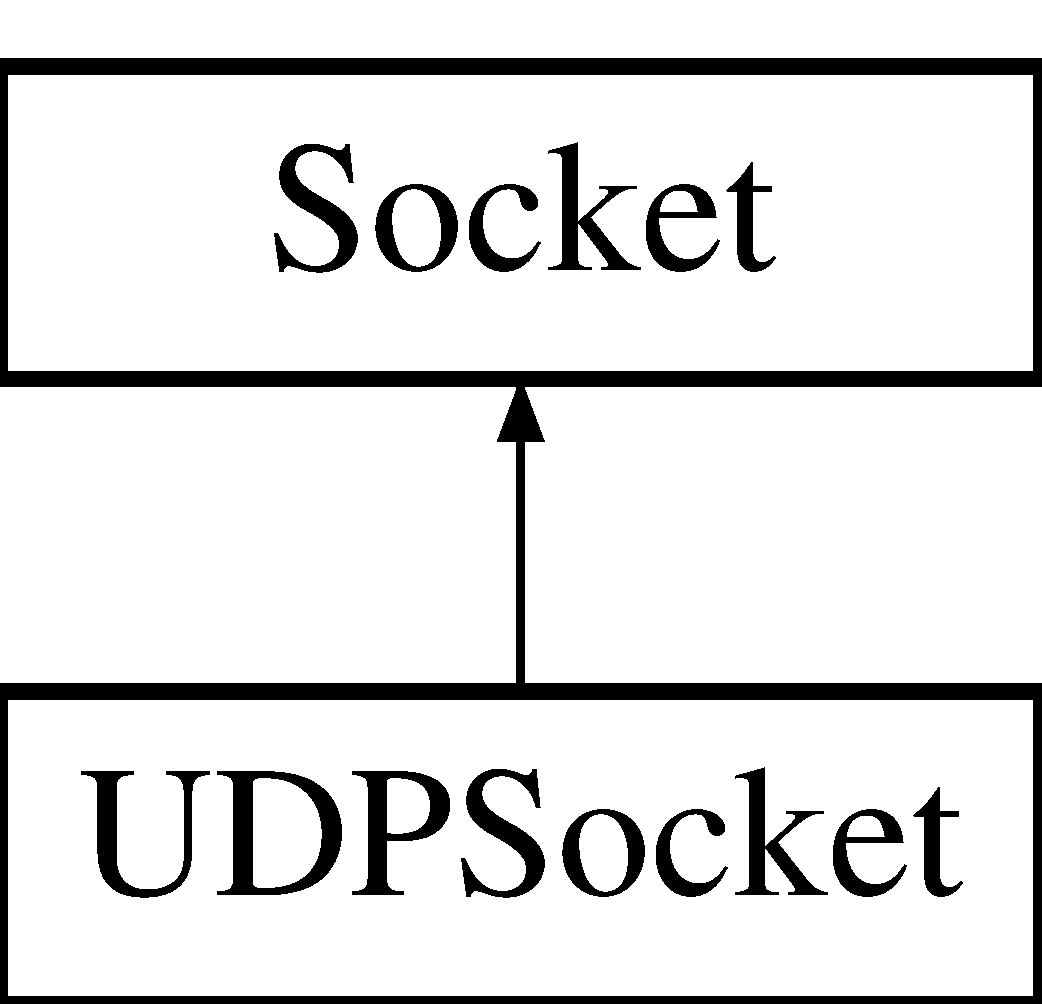
\includegraphics[height=2cm]{classUDPSocket}
\end{center}
\end{figure}
\subsection*{Public Member Functions}
\begin{CompactItemize}
\item 
\hyperlink{classUDPSocket_7e2e6eb3a4c3eec5538bdfd89441802b}{UDPSocket} (int \hyperlink{classSocket_c7f6980f36023df2004271c336217cb8}{type}=AF\_\-INET)  throw ()
\begin{CompactList}\small\item\em \hyperlink{classUDPSocket}{UDPSocket} constructor. \item\end{CompactList}\item 
void \hyperlink{classUDPSocket_28db3dc93452723bdfd861442268b87c}{send} (const std::string \&buf, const std::string \&host, u\_\-int16\_\-t port)  throw ()
\begin{CompactList}\small\item\em Send a string onto an UDP socket. \item\end{CompactList}\item 
void \hyperlink{classUDPSocket_254a2df8f7205266cd684931e9914ba9}{send} (const void $\ast$buf, u\_\-int32\_\-t size, const std::string \&host, u\_\-int16\_\-t port)  throw ()
\begin{CompactList}\small\item\em Send a binary buffer onto an UDP socket. \item\end{CompactList}\item 
void \hyperlink{classUDPSocket_93ca497a5e6539eab464c4bd59a85de2}{bind} (u\_\-int16\_\-t port)  throw ()
\begin{CompactList}\small\item\em Bind an UDP socket onto a port. \item\end{CompactList}\item 
void \hyperlink{classUDPSocket_5ee2f9411fad95d5bc7ebd3eecb7d86f}{recv} (void $\ast$buf, u\_\-int32\_\-t size, const std::string \&host=\char`\"{}\char`\"{}, u\_\-int16\_\-t port=0)  throw ()
\begin{CompactList}\small\item\em Receive a binary buffer from an UDP socket. \item\end{CompactList}\item 
std::string \hyperlink{classUDPSocket_688933363fb0b6b9819234dcfe13931b}{recv} (const std::string \&host=\char`\"{}\char`\"{}, u\_\-int16\_\-t port=0)  throw ()
\begin{CompactList}\small\item\em Receive an ASCII string from an UDP socket. \item\end{CompactList}\item 
std::string \hyperlink{classUDPSocket_212e096b3245ea32b66f43c592903838}{readline} (const std::string \&host=\char`\"{}\char`\"{}, u\_\-int16\_\-t port=0)  throw ()
\begin{CompactList}\small\item\em Read an ASCII line from an UDP socket. \item\end{CompactList}\end{CompactItemize}


\subsection{Detailed Description}
Class for managing UDP sockets. 

\begin{Desc}
\item[Author:]BlackLight \end{Desc}


\subsection{Constructor \& Destructor Documentation}
\hypertarget{classUDPSocket_7e2e6eb3a4c3eec5538bdfd89441802b}{
\index{UDPSocket@{UDPSocket}!UDPSocket@{UDPSocket}}
\index{UDPSocket@{UDPSocket}!UDPSocket@{UDPSocket}}
\subsubsection[{UDPSocket}]{\setlength{\rightskip}{0pt plus 5cm}UDPSocket::UDPSocket (int {\em type} = {\tt AF\_\-INET})  throw ()}}
\label{classUDPSocket_7e2e6eb3a4c3eec5538bdfd89441802b}


\hyperlink{classUDPSocket}{UDPSocket} constructor. 

\begin{Desc}
\item[Parameters:]
\begin{description}
\item[{\em type}]\hyperlink{classSocket}{Socket} type (default = AF\_\-INET) \end{description}
\end{Desc}


\subsection{Member Function Documentation}
\hypertarget{classUDPSocket_93ca497a5e6539eab464c4bd59a85de2}{
\index{UDPSocket@{UDPSocket}!bind@{bind}}
\index{bind@{bind}!UDPSocket@{UDPSocket}}
\subsubsection[{bind}]{\setlength{\rightskip}{0pt plus 5cm}void UDPSocket::bind (u\_\-int16\_\-t {\em port})  throw ()}}
\label{classUDPSocket_93ca497a5e6539eab464c4bd59a85de2}


Bind an UDP socket onto a port. 

\begin{Desc}
\item[Parameters:]
\begin{description}
\item[{\em Port}]\end{description}
\end{Desc}
\hypertarget{classUDPSocket_212e096b3245ea32b66f43c592903838}{
\index{UDPSocket@{UDPSocket}!readline@{readline}}
\index{readline@{readline}!UDPSocket@{UDPSocket}}
\subsubsection[{readline}]{\setlength{\rightskip}{0pt plus 5cm}std::string UDPSocket::readline (const std::string \& {\em host} = {\tt \char`\"{}\char`\"{}}, \/  u\_\-int16\_\-t {\em port} = {\tt 0})  throw ()}}
\label{classUDPSocket_212e096b3245ea32b66f43c592903838}


Read an ASCII line from an UDP socket. 

\begin{Desc}
\item[Parameters:]
\begin{description}
\item[{\em host}]Remote host name/address \item[{\em port}]Remote port \end{description}
\end{Desc}
\begin{Desc}
\item[Returns:]String received \end{Desc}
\hypertarget{classUDPSocket_688933363fb0b6b9819234dcfe13931b}{
\index{UDPSocket@{UDPSocket}!recv@{recv}}
\index{recv@{recv}!UDPSocket@{UDPSocket}}
\subsubsection[{recv}]{\setlength{\rightskip}{0pt plus 5cm}std::string UDPSocket::recv (const std::string \& {\em host} = {\tt \char`\"{}\char`\"{}}, \/  u\_\-int16\_\-t {\em port} = {\tt 0})  throw ()}}
\label{classUDPSocket_688933363fb0b6b9819234dcfe13931b}


Receive an ASCII string from an UDP socket. 

\begin{Desc}
\item[Parameters:]
\begin{description}
\item[{\em host}]Remote host name/address \item[{\em port}]Remote port \end{description}
\end{Desc}
\begin{Desc}
\item[Returns:]String received \end{Desc}
\hypertarget{classUDPSocket_5ee2f9411fad95d5bc7ebd3eecb7d86f}{
\index{UDPSocket@{UDPSocket}!recv@{recv}}
\index{recv@{recv}!UDPSocket@{UDPSocket}}
\subsubsection[{recv}]{\setlength{\rightskip}{0pt plus 5cm}void UDPSocket::recv (void $\ast$ {\em buf}, \/  u\_\-int32\_\-t {\em size}, \/  const std::string \& {\em host} = {\tt \char`\"{}\char`\"{}}, \/  u\_\-int16\_\-t {\em port} = {\tt 0})  throw ()}}
\label{classUDPSocket_5ee2f9411fad95d5bc7ebd3eecb7d86f}


Receive a binary buffer from an UDP socket. 

\begin{Desc}
\item[Parameters:]
\begin{description}
\item[{\em buf}]Buffer where we're going to place our data \item[{\em size}]Number of bytes to be read \item[{\em host}]Remote host name/address \item[{\em port}]Remote port \end{description}
\end{Desc}
\hypertarget{classUDPSocket_254a2df8f7205266cd684931e9914ba9}{
\index{UDPSocket@{UDPSocket}!send@{send}}
\index{send@{send}!UDPSocket@{UDPSocket}}
\subsubsection[{send}]{\setlength{\rightskip}{0pt plus 5cm}void UDPSocket::send (const void $\ast$ {\em buf}, \/  u\_\-int32\_\-t {\em size}, \/  const std::string \& {\em host}, \/  u\_\-int16\_\-t {\em port})  throw ()}}
\label{classUDPSocket_254a2df8f7205266cd684931e9914ba9}


Send a binary buffer onto an UDP socket. 

\begin{Desc}
\item[Parameters:]
\begin{description}
\item[{\em buf}]Binary buffer to be sent \item[{\em size}]buf's size \item[{\em host}]Remote host name/address \item[{\em port}]Remote port \end{description}
\end{Desc}
\hypertarget{classUDPSocket_28db3dc93452723bdfd861442268b87c}{
\index{UDPSocket@{UDPSocket}!send@{send}}
\index{send@{send}!UDPSocket@{UDPSocket}}
\subsubsection[{send}]{\setlength{\rightskip}{0pt plus 5cm}void UDPSocket::send (const std::string \& {\em buf}, \/  const std::string \& {\em host}, \/  u\_\-int16\_\-t {\em port})  throw ()}}
\label{classUDPSocket_28db3dc93452723bdfd861442268b87c}


Send a string onto an UDP socket. 

\begin{Desc}
\item[Parameters:]
\begin{description}
\item[{\em buf}]String to be sent \item[{\em host}]Remote host name/address \item[{\em port}]Remote port \end{description}
\end{Desc}


The documentation for this class was generated from the following file:\begin{CompactItemize}
\item 
\hyperlink{usock_8h}{usock.h}\end{CompactItemize}

\chapter{File Documentation}
\hypertarget{usock_8h}{
\section{usock.h File Reference}
\label{usock_8h}\index{usock.h@{usock.h}}
}
{\tt \#include $<$string$>$}\par
\subsection*{Classes}
\begin{CompactItemize}
\item 
struct \hyperlink{structicmp__hdr}{icmp\_\-hdr}
\item 
struct \hyperlink{structpseudohdr}{pseudohdr}
\item 
class \hyperlink{classSocket}{Socket}
\begin{CompactList}\small\item\em Base socket class for building, by default, TCP sockets. \item\end{CompactList}\item 
class \hyperlink{classServerSocket}{ServerSocket}
\begin{CompactList}\small\item\em Class for managing server sockets. \item\end{CompactList}\item 
class \hyperlink{classUDPSocket}{UDPSocket}
\begin{CompactList}\small\item\em Class for managing UDP sockets. \item\end{CompactList}\item 
class \hyperlink{classRawSocket}{RawSocket}
\begin{CompactList}\small\item\em Class for managing raw sockets. \item\end{CompactList}\end{CompactItemize}
\subsection*{Defines}
\begin{CompactItemize}
\item 
\#define \hyperlink{usock_8h_29d0df17f4d361506734c2083f200ea3}{BUFRECV\_\-SIZE}~1024
\item 
\#define \hyperlink{usock_8h_fb2b62b61a722c73b8b798f010063863}{DEFAULT\_\-MAXCON}~10
\item 
\#define \hyperlink{usock_8h_1cec9b372679734fcd8394d779442ddb}{TH\_\-FIN}~0x01
\item 
\#define \hyperlink{usock_8h_91006117f7ae427b957773ab0e80bfa4}{TH\_\-SYN}~0x02
\item 
\#define \hyperlink{usock_8h_7f2ce15991898c8d3397045087c4381f}{TH\_\-RST}~0x04
\item 
\#define \hyperlink{usock_8h_45b9964096064c9a0c84fbddd2c80d38}{TH\_\-PUSH}~0x08
\item 
\#define \hyperlink{usock_8h_362dae974cf06bab2b79b70f0cde524f}{TH\_\-ACK}~0x10
\item 
\#define \hyperlink{usock_8h_7b18ca973f14696013696a00c5235f32}{TH\_\-URG}~0x20
\end{CompactItemize}


\subsection{Define Documentation}
\hypertarget{usock_8h_29d0df17f4d361506734c2083f200ea3}{
\index{usock.h@{usock.h}!BUFRECV\_\-SIZE@{BUFRECV\_\-SIZE}}
\index{BUFRECV\_\-SIZE@{BUFRECV\_\-SIZE}!usock.h@{usock.h}}
\subsubsection[{BUFRECV\_\-SIZE}]{\setlength{\rightskip}{0pt plus 5cm}\#define BUFRECV\_\-SIZE~1024}}
\label{usock_8h_29d0df17f4d361506734c2083f200ea3}


====================================== \_\- \_\- \_\- \_\- $|$ (\_\-) $|$ $|$ $|$ $|$ $|$\_\-$|$ $|$\_\-\_\- \_\- \_\- \_\-\_\-\_\- \_\-\_\-\_\- \_\-\_\-\_\-$|$ $|$ \_\-\_\- $|$ $|$ $|$ '\_\- $\backslash$$|$ $|$ $|$ / \_\-\_\-$|$/ \_\- $\backslash$ / \_\-\_\-$|$ $|$/ / $|$ $|$ $|$ $|$\_\-) $|$ $|$\_\-$|$  $\backslash$ (\_\-) $|$ (\_\-\_\-$|$ $<$ $|$\_\-$|$\_\-$|$\_\-.\_\-\_\-/ ,\_\-$|$\_\-\_\-\_\-// $|$\_\-$|$$\backslash$

======================================

The files in this directory and elsewhere which refer to this LICENCE file are part of uSock, the library for the high-level management of network sockets.

Copyright (C) 2009 by BlackLight, $<$\href{mailto:blacklight@autistici.org}{\tt blacklight@autistici.org}$>$ Web: \href{http://0x00.ath.cx}{\tt http://0x00.ath.cx}

uSock is free software; you can redistribute it and/or modify it under the terms of the GNU General Public License as published by the Free Software Foundation; either version 3 or (at your option) any later version.

uSock is distributed in the hope that it will be useful, but WITHOUT ANY WARRANTY; without even the implied warranty of MERCHANTABILITY or FITNESS FOR A PARTICULAR PURPOSE. See the GNU General Public License for more details.

You should have received a copy of the GNU General Public License along with uSock; if not, write to the Free Software Foundation, Inc., 59 Temple Place, Suite 330, Boston, MA 02111-1307 USA.

As a special exception, if other files instantiate templates or use macros or inline functions from these files, or you compile these files and link them with other works to produce a work based on these files, these files do not by themselves cause the resulting work to be covered by the GNU General Public License. However the source code for these files must still be made available in accordance with section (3) of the GNU General Public License.

This exception does not invalidate any other reasons why a work based on this file might be covered by the GNU General Public License. \hypertarget{usock_8h_fb2b62b61a722c73b8b798f010063863}{
\index{usock.h@{usock.h}!DEFAULT\_\-MAXCON@{DEFAULT\_\-MAXCON}}
\index{DEFAULT\_\-MAXCON@{DEFAULT\_\-MAXCON}!usock.h@{usock.h}}
\subsubsection[{DEFAULT\_\-MAXCON}]{\setlength{\rightskip}{0pt plus 5cm}\#define DEFAULT\_\-MAXCON~10}}
\label{usock_8h_fb2b62b61a722c73b8b798f010063863}


\hypertarget{usock_8h_362dae974cf06bab2b79b70f0cde524f}{
\index{usock.h@{usock.h}!TH\_\-ACK@{TH\_\-ACK}}
\index{TH\_\-ACK@{TH\_\-ACK}!usock.h@{usock.h}}
\subsubsection[{TH\_\-ACK}]{\setlength{\rightskip}{0pt plus 5cm}\#define TH\_\-ACK~0x10}}
\label{usock_8h_362dae974cf06bab2b79b70f0cde524f}


\hypertarget{usock_8h_1cec9b372679734fcd8394d779442ddb}{
\index{usock.h@{usock.h}!TH\_\-FIN@{TH\_\-FIN}}
\index{TH\_\-FIN@{TH\_\-FIN}!usock.h@{usock.h}}
\subsubsection[{TH\_\-FIN}]{\setlength{\rightskip}{0pt plus 5cm}\#define TH\_\-FIN~0x01}}
\label{usock_8h_1cec9b372679734fcd8394d779442ddb}


\hypertarget{usock_8h_45b9964096064c9a0c84fbddd2c80d38}{
\index{usock.h@{usock.h}!TH\_\-PUSH@{TH\_\-PUSH}}
\index{TH\_\-PUSH@{TH\_\-PUSH}!usock.h@{usock.h}}
\subsubsection[{TH\_\-PUSH}]{\setlength{\rightskip}{0pt plus 5cm}\#define TH\_\-PUSH~0x08}}
\label{usock_8h_45b9964096064c9a0c84fbddd2c80d38}


\hypertarget{usock_8h_7f2ce15991898c8d3397045087c4381f}{
\index{usock.h@{usock.h}!TH\_\-RST@{TH\_\-RST}}
\index{TH\_\-RST@{TH\_\-RST}!usock.h@{usock.h}}
\subsubsection[{TH\_\-RST}]{\setlength{\rightskip}{0pt plus 5cm}\#define TH\_\-RST~0x04}}
\label{usock_8h_7f2ce15991898c8d3397045087c4381f}


\hypertarget{usock_8h_91006117f7ae427b957773ab0e80bfa4}{
\index{usock.h@{usock.h}!TH\_\-SYN@{TH\_\-SYN}}
\index{TH\_\-SYN@{TH\_\-SYN}!usock.h@{usock.h}}
\subsubsection[{TH\_\-SYN}]{\setlength{\rightskip}{0pt plus 5cm}\#define TH\_\-SYN~0x02}}
\label{usock_8h_91006117f7ae427b957773ab0e80bfa4}


\hypertarget{usock_8h_7b18ca973f14696013696a00c5235f32}{
\index{usock.h@{usock.h}!TH\_\-URG@{TH\_\-URG}}
\index{TH\_\-URG@{TH\_\-URG}!usock.h@{usock.h}}
\subsubsection[{TH\_\-URG}]{\setlength{\rightskip}{0pt plus 5cm}\#define TH\_\-URG~0x20}}
\label{usock_8h_7b18ca973f14696013696a00c5235f32}



\hypertarget{usock__exception_8h}{
\section{usock\_\-exception.h File Reference}
\label{usock__exception_8h}\index{usock\_\-exception.h@{usock\_\-exception.h}}
}
{\tt \#include $<$exception$>$}\par
{\tt \#include $<$cerrno$>$}\par
\subsection*{Classes}
\begin{CompactItemize}
\item 
class \hyperlink{classusock_1_1SocketException}{usock::SocketException}
\begin{CompactList}\small\item\em Class for managing exceptions in \hyperlink{namespaceusock}{usock} class. \item\end{CompactList}\end{CompactItemize}
\subsection*{Namespaces}
\begin{CompactItemize}
\item 
namespace \hyperlink{namespaceusock}{usock}
\end{CompactItemize}
\subsection*{Defines}
\begin{CompactItemize}
\item 
\#define \hyperlink{usock__exception_8h_8aa7a302e0160545c42054cfa6e3b743}{ERRBUF\_\-SIZE}~1024
\end{CompactItemize}


\subsection{Define Documentation}
\hypertarget{usock__exception_8h_8aa7a302e0160545c42054cfa6e3b743}{
\index{usock\_\-exception.h@{usock\_\-exception.h}!ERRBUF\_\-SIZE@{ERRBUF\_\-SIZE}}
\index{ERRBUF\_\-SIZE@{ERRBUF\_\-SIZE}!usock_exception.h@{usock\_\-exception.h}}
\subsubsection[{ERRBUF\_\-SIZE}]{\setlength{\rightskip}{0pt plus 5cm}\#define ERRBUF\_\-SIZE~1024}}
\label{usock__exception_8h_8aa7a302e0160545c42054cfa6e3b743}



\printindex
\end{document}
